% \subsection{Redes neuronales artificiales - \textit{Artificial Neuronal Networks}}
\subsection[\texorpdfstring{Redes neuronales artificiales \\ \textit{Artificial Neuronal Networks}}{Redes neuronales artificiales - Artificial Neuronal Networks}]{Redes neuronales artificiales \\ \textit{Artificial Neuronal Networks}}
% region subsection Redes neuronales artificiales
% TODO: \cite{ibm-deep-learning}
% Explicar uso de múltiples neuronas artificiales para crear capas y luego redes
El \textit{deep learning} emplea principalmente redes neuronales para reconocer, clasificar y describir con precisión patrones de datos. Estas redes están inspiradas en el funcionamiento del cerebro humano.  \cite{ibm-deep-learning}

Las redes neuronales es un conjunto de neuronas artificiales que están organizadas generalmente por capas. Estas redes tienen una capa de entrada, una capa de salida y múltiples capas ocultas con distintas funciones de activación que ponderan los pesos de cada neurona.

Existen formas muy variadas de componer las capas, a esto se le denomina \textbf{topología de red neuronal}, en función del objetivo que se busque, la topología será muy distinta.

\subsubsection{Elementos de una neurona artificial}
% region subsubsection Elementos de una neurona artificial
% TODO explicar las partes que propusieron \textit{McCulloch} y \textit{Pitts}

Como se ha comentado previamente las neuronas artificiales están inspiradas en las neuronas biológicas del cerebro humano, fueron los investigadores \textit{McCulloch} y \textit{Pitts} \cite{mcculloch1943logical} los que sentaron las bases de lo que es una neurona artificial, demostrando que su modelo de red neuronal podía realizar cálculos que se correspondían con la lógica proposicional.


\begin{figure}[H]
    \centering
    \centerline{\includesvg[width=0.99\linewidth]{figures/chapter02/artificial-neuron.drawio.svg}}
    \caption{Partes de una neurona artificial bioinspirada en una neurona biológica.\newline{}Fuente: Elaboración propia.}
    \label{fig:artificial-neuron}
\end{figure}

En la Figura \ref{fig:artificial-neuron} podemos ver las distintas partes de una única neurona artificial y sus partes equivalentes con una neurona biológica. El axón opera como la entrada de información a la neurona. La sinapsis como las conexiones con la neurona que son los pesos. El cuerpo celular como la unidad de procesamiento central, donde se pondera la suma de las señales de entrada. El cuello del axón sería nuestra función de activación que se activa cuando supera un umbral. Y por último el axón sería nuestra señal de salida.



% perceptron simple
% perceptron multicapa
% Funciones de optimización
% Funciones de activación
% Funciones de perdida
% CapasThe next payment of €9.68 will be collected on March 13th, 2024 10:26 AM UTC.

% Tipologías
% Descenso de gradiente

% endregion subsubsection Elementos de una neurona artificial

\subsubsection{Funcionamiento de una red neuronal} \label{neural-network}
% region subsubsection Funcionamiento de una red neuronal

Las redes neuronales profundas tienen multitud de capas con nodos interconectados, cada capa sobre la capa anterior con el objetivo de optimizar la precisión de una perdición o clasificación. A esta progresión de cálculos se le denomina ``propagación hacia delante''.

El proceso de ``propagación inversa'' es el encargado de calcular errores de precisión, ajustar sesgos y ponderaciones usando algoritmos como \nameref{sec:gradient-descent}.

La capa de entrada es por donde el modelo ingiere los datos, y la capa de salida es donde el modelo responderá con la predicción o clasificación una vez se haya completado la fase de aprendizaje.

\begin{figure}[H]
    \centering
    \centerline{\includesvg[width=0.99\linewidth]{figures/chapter02/neuronal-network.drawio.svg}}
    \caption{Red neuronal artificial.\newline{}Fuente: Elaboración propia.}
    \label{fig:artificial-neuronal-network}
\end{figure}

En la Figura \ref{fig:artificial-neuronal-network} podemos ver una arquitectura simple de una red neuronal que cuenta con la capa de entrada, la capa de salida y dos capas ocultas.

El vector de entrada ${X = (x_{1}, x_{2}, ..., x_{n})}$ será la información suministrada a nuestra red a través de la capa de entrada, este vector será de tamaño ${n}$.

\begin{figure}[H]
    \centering
    \captionsetup{justification=centering}
    \centerline{\includesvg[width=0.99\linewidth]{figures/equations/Notation.drawio.svg}}
    \caption{Cálculo de los pesos de la red neuronal artificial.\newline{}Fuente: Elaboración propia.}
    \label{fig:notation}
\end{figure}

\clearpage

\begin{enumerate}
    \item Función de la red neuronal: ${f(x) = W x + b}$
    \item Matriz de pesos: ${W = \left[w_{0,n}, w_{1,n}, ...,w_{m,n}\right]}$
    \item Vector de pesos: ${w_{n} \in \mathbb{R}^{D}}$
    \item Vector de entrada: ${x \in \mathbb{R}^{D}}$
    \item Vector del bias: ${b \in \mathbb{R}^{C}}$
\end{enumerate}

% El proceso de reducción de dimensionalidad se lleva a cabo, para convertir el vector de características del espacio original en un nuevo espacio con un conjunto más pequeño, linealmente no correlacionadas mediante la siguiente función $f: \mathbb{R}^{D} \rightarrow \mathbb{R}^{C}$ con $C \ll D$, donde la red neuronal está expresada como $f(x) = W x + b$. Esta red cuenta con las siguientes partes $\mathbf{W} = \left[w_{0}^{T}, w_{1}^{T}, \cdots, w_{C}^{T}\right]$ es la matriz de vectores de peso, que viene dada la expresión $\mathbf{w_{j}} \in \mathbb{R}^{D}$. El vector de entrada es $\mathbf{x} \in \mathbb{R}^{D}$ y el $bias$ es un vector que está definido en el espacio $\mathbf{b} \in \mathbb{R}^{C}$

\paragraph*{El perceptrón simple}
% TODO: Definición
% TODO: Usos 
% TODO: Algoritmo de entranmiento
% TODO: Problema XOR

El Perceptron es una neurona artificial simple llamada también como \gls{LTU}. La \gls{LTU} calcula una suma ponderada de los valores de las entradas, ${Z = w_{1} x_{1} + w_{2} x_{2} + \cdots + w_{n} x_{n}}$ se aplica el umbral para generar el resultado.

La función umbral común en \gls{LTU} es la función Heaviside \ref{eq:heaviside}.

\noindent\begin{minipage}{0.45\textwidth}
    \begin{equation*}
        heaviside(z) =
        \begin{cases}
            0 & \textup{si } z < 0       \\
            1 & \textup{si } z \geq{}  0
        \end{cases}
    \end{equation*}
\end{minipage}
\begin{minipage}{0.45\textwidth}
    \begin{equation}
        sgn(z) =
        \begin{cases}
            -1 & \textup{si } z < 0  \\
            0  & \textup{si } z = 0  \\
            +1 & \textup{si } z >  0
        \end{cases}
        \label{eq:heaviside}
    \end{equation}
\end{minipage}

Se puede emplear para una clasificación binaria lineal simple, mediante una combinación lineal de las entradas; si la operación supera el umbral, se obtendrá un resultado binario en un vector.

El algoritmo de entrenamiento del perceptrón se basa en ajustar los pesos de conexión entre las entradas y la neurona de salida para mejorar la precisión de las predicciones. Está inspirado en la regla de Hebb, que sugiere que las conexiones entre neuronas se fortalecen cuando una neurona activa repetidamente a otra.

Primero inicializa los pesos, predice, evalúa su error y actualización de los pesos para en la siguiente iteración minimizar su error.

Rosenblatt demostró que el algoritmo convergería hacia una solución, esto es llamado el Teorema de convergencia del perceptrón \cite{geron2018neural}.

Marvin Minsky y Seymour encontraron una serie de debilidades que los perceptrones son incapaces de resolver, algunas de estas debilidades se pueden resolver apilando varios perceptrones, la \acrshort{ANN} resultante se le denomina \gls{MLP}.

Uno de los problemas clásicos que tenían los perceptrones simples era el problema de clasificación XOR, esto está representado en la Figura \ref{fig:problem-xor}. Como tal, el perceptrón es un modelo que puede aprender funciones lineales, pero el problema XOR no es linealmente separable, lo que significa que no se puede trazar una línea recta para separar las dos clases (A y B) en el espacio de entrada binario de dos dimensiones.

\begin{figure}[H]
    \centering
    \centerline{\includesvg[width=0.35\linewidth]{figures/chapter02/tfm-xor-problem.drawio.svg}}
    \caption{Problema de clasificación XOR.\newline{}Fuente: Elaboración propia.}
    \label{fig:problem-xor}
\end{figure}


\paragraph*{El perceptrón multicapa y retropropagación}

Fue en 1986 cuando {D. E. Rumelhart} propuso la retro propagación junto a múltiples capas para resolver el problema de clasificación XOR.

El proceso es el siguiente, por cada instancia de entrenamiento se calcula la salida de cada neurona en la capa consecutiva (paso hacia adelante). A continuación se mide el error de salida de la red (la diferencia entre la salida deseada y la de la red) calculará cuánto contribuyo cada neurona en la última capa oculta al error de cada neurona de salida. Se mide cuantas contribuciones de error provienen de cada neurona en la capa oculta anterior, así sucesivamente hasta que se llega a la capa de entrada(paso hacia atrás). Se mide eficientemente el gradiente de error en todos los pesos de la conexión en la red propagando el gradiente de error hacia atrás. \cite{geron2018neural}

Este proceso funciona, ya que se cambió la función escalonada de las \gls{LTU} a una función logística Sigmoid, esto se requería, ya que la función de paso contiene solo segmentos planos y, por tanto, no había gradientes. Esto permitió que el descenso de gradiente pudiera ir progresando lentamente hasta converger. El algoritmo de retroalimentación se puede usar con otras funciones de activación que veremos más adelante.

% endregion subsubsection Funcionamiento de una red neuronal

\subsubsection{El descenso de gradiente} \label{sec:gradient-descent}
% region El descenso de gradiente
% README: https://www.ibm.com/mx-es/topics/gradient-descent
% TODO: definición
% TODO: como funciona 
% TODO: tipos de descenso
% TODO: desafios (problema)

El método de descenso de gradiente trata de encontrar un mínimo en una función dada, ya sea local o global. El método usa el gradiente negativo ${-\nabla{f}}$, con este método obtenemos la dirección con el descenso máximo en los valores de la función, con esto buscamos encontrar la posición mínima.

En términos simples, el descenso de gradiente va ajustando iterativamente los valores de los parámetros en la dirección opuesta al gradiente de la función de costo. Al moverse en la dirección opuesta al gradiente, el algoritmo busca alcanzar el mínimo local o global de la función de costo.

\begin{figure}[H]
    \centering
    \centerline{\includesvg[width=0.6\linewidth]{figures/chapter02/fx_optimizer.svg}}
    \caption{Descenso de gradiente.\newline{}Fuente: \href{https://fxdatalabs.com}{F(x) Data Labs Pvt. Ltd.}}
    \label{fig:gradient-descent}
\end{figure}

\begin{algorithm}[H]
    \SetAlgoLined
    \DontPrintSemicolon
    Seleccionar ${x^{(0)}}$\;
    Establecer ${k \leftarrow 0}$\;
    \While{${ \left\lVert \nabla f(x^{(k)}) \right\rVert \geq \epsilon }$} {
        ${x^{(k+1)} = x^{k} - t_{k} - t_{k} \nabla f(x^{(k)})}$\;
        ${k \leftarrow k + 1}$\;
    }
    \Return{${x^{(k)}}$}\;
    \label{alg:plot-gradient-descent}
    \caption{Descenso de gradiente}
\end{algorithm}

Hay tres variantes del algoritmo de aprendizaje del descenso de gradiente \cite{ibm-gradient-descent}.

\begin{itemize}
    \item \textbf{Descenso de gradiente por lotes}: suma el error para cada punto en un conjunto de entrenamiento, actualiza el modelo después de que todos los ejemplos de entrenamiento han sido evaluados, esto es lo que se le conoce como épocas. Es un método eficiente computacionalmente, pero costoso para grandes conjuntos de datos, ya que requiere almacenar en memoria todos los datos, suele producir un gradiente de error estable y una convergencia, pero a veces ese punto de convergencia no es el ideal y encuentra el mínimo local frente al global.
    \item \textbf{Descenso de gradiente estocástico}: en cada época actualiza los parámetros del ejemplo de entrenamiento, esto reduce la necesidad de memoria, la actualización proporciona velocidad y detalles, aunque requieren un coste computacional mayor. Los gradientes son más ruidosos por sus actualizaciones frecuentes, esto le permite salir de mínimos locales.
    \item \textbf{Descenso de gradiente por mini lotes}: combina aspectos de del descenso de gradiente por lotes como el estocástico. Divide el conjunto de entrenamiento en pequeños lotes y realiza actualizaciones en cada uno de estos lotes. Esto permite tener un equilibrio entre eficiencia computacional y velocidad del descenso de gradiente.
\end{itemize}


% \begin{table}[H]
%     \centering
%     \footnotesize
%     \begin{tabularx}{\textwidth}{|p{3cm}|>{\raggedright\arraybackslash}X|X|X|}\hline
%         \textbf{Aspecto}              & \textbf{Descenso de Gradiente por Lotes}           & \textbf{Descenso de Gradiente Estocástico}           & \textbf{Descenso de Gradiente por Mini Lotes}   \\\hline
%         Eficiencia computacional      & Eficiente para conjuntos de datos pequeños.        & Menos eficiente para grandes conjuntos de datos.     & Equilibrio entre eficiencia y velocidad.        \\\hline
%         Coste computacional           & Puede ser lento para grandes conjuntos de datos.   & Más rápido que por lotes, pero aún puede ser lento.  & Mejor tiempo de procesamiento que por lotes.    \\\hline
%         Coste en memoria              & Requiere almacenar todo el conjunto en memoria.    & Solo necesita almacenar un ejemplo a la vez.         & Menos demandante que por lotes, pero eficiente. \\\hline
%         Convergencia del Modelo       & Propenso a converger hacia mínimos locales.        & Puede saltar mínimos locales pero es ruidoso.        & Convergencia más estable que SGD, menos ruido.  \\\hline
%         Sensibilidad a datos ruidosos & Menos sensible debido al promedio de errores.      & Más sensible debido a actualizaciones frecuentes.    & Menos sensible que SGD, gracias al promedio.    \\\hline
%         Tamaño del conjunto de datos  & Funciona bien para conjuntos de datos pequeños.    & Buen rendimiento para distintos tamaños.             & Equilibrio, adecuado para diferentes tamaños.   \\\hline
%         Precisión del modelo          & Convergencia más estable, pero a veces sub óptima. & Puede converger más rápidamente, pero menos estable. & Balance entre estabilidad y rapidez.            \\\hline
%     \end{tabularx}
%     \caption{Tabla comparativa de los tipos de descenso de gradiente}
%     \label{tab:tabla-comparativa}
% \end{table}

% \paragraph*{Problema de mínimos locales y puntos de silla}
% TODO: no creo que sea necesario explicar mínimos locales y puntos de silla.

\paragraph*{Problema de desvanecimiento y explosión de gradiente}
Hablaremos primero del desvanecimiento de gradiente, esto ocurre durante la retro propagación, ya que al movernos hacia atrás el gradiente sigue haciéndose más pequeño, esto hace que las capas anteriores de la red aprendan más lentamente que las posteriores. A medida que el algoritmo itera los cambios se hacen insignificantes, lo que hace que el algoritmo se estanque.

El problema de la explosión de gradiente es lo contrario, el gradiente se hace demasiado grande creando un modelo inestable. Los pesos del modelo crecerán y eventualmente se representarán como \texttt{NaN}.

% Escribe esto de forma que no sea una copia de ibm, está perfectamente explicado, pero no puede ser una copia :3
% \textbf{Desaparición de gradientes}: esto ocurre cuando el gradiente es demasiado pequeño. A medida que nos movemos hacia atrás durante la retropropagación, el gradiente continúa haciéndose más pequeño, lo que hace que las capas anteriores de la red aprendan más lentamente que las capas posteriores. Cuando esto sucede, los parámetros de peso se actualizan hasta que se vuelven insignificantes, es decir, 0, lo que genera un algoritmo que ya no está aprendiendo.
% \textbf{Explosión de gradientes}: esto sucede cuando el gradiente es demasiado grande, creando un modelo inestable. En este caso, los pesos del modelo crecerán demasiado y eventualmente se representarán como NaN. Una solución a este problema es aprovechar una técnica de reducción de dimensionalidad, que puede ayudar a minimizar la complejidad dentro del modelo.


% \begin{figure}[H]
%     \begin{subfigure}{.475\linewidth}
%         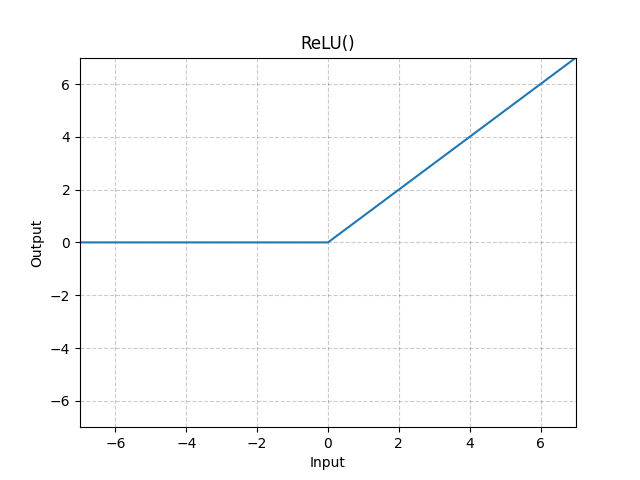
\includegraphics[width=\linewidth]{figures/equations/ReLU.png}
%         \caption{}
%         \label{subfig:funcion-minimo-local}
%     \end{subfigure}\hfill % <-- \hfill
%     \begin{subfigure}{.475\linewidth}
%         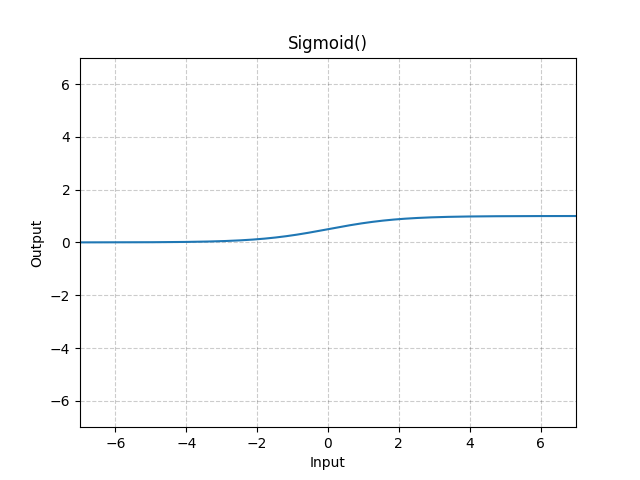
\includegraphics[width=\linewidth]{figures/equations/Sigmoid.png}
%         \caption{}
%         \label{subfig:funcion-punto-de-silla}
%     \end{subfigure}
%     \caption{Mínimos locales y puntos de silla}
%     \label{fig:locales}
% \end{figure}

% endregion El descenso de gradiente

\subsubsection{Optimizadores} \label{optimizers}
% region Optimizadores
% TODO: definición
% TODO: Tipos
% TODO: Usos
Los optimizadores son los algoritmos que buscan encontrar la mejor solución para un problema, esto se utilizan en conjunto con el descenso de gradiente para mejorar su eficiencia y rendimiento, generalmente minimizando o maximizando una función objetiva al ajustar sus parámetros. Existen muchos optimizadores que nos permiten explorar de forma eficiente el espacio de posibles soluciones.

% https://interactivechaos.com/es/manual/tutorial-de-machine-learning/adagrad

Estos son algunos de los optimizadores más famosos.
\begin{enumerate}
    \item \textbf{SGD} (Stochastic Gradient Descent with Momentum): Descenso de gradiente estocástico con momentum.
    \item \textbf{Adam} (Adaptive Moment Estimation): Descenso de gradiente con tasa de aprendizaje adaptativa.
    \item \textbf{Adamax} (Adaptive Moment Estimation with Infinity Norm):  variante de Adam que utiliza la norma infinita en lugar de la norma 2 para calcular y actualizar el término de escala máximo.
    \item \textbf{AdaGrad} (Adaptative Gradient Algorithm): variante de \textit{SGD} en la que se emplean distintas tasas de aprendizaje teniendo en cuenta el gradiente acumulado en cada una de las variables.
    \item \textbf{RMSprop} (Root Mean Square Propagation): variante de \textit{AdaGrad} en la que, en lugar de mantener un acumulado los gradientes, se utiliza el concepto de ``ventana'' para considerar los gradientes más recientes.
\end{enumerate}

% endregion Optimizadore

\subsubsection{Funciones de activación} \label{sec:activations-functions}
% region Funciones de activación
% TODO: definición, explicación y usos
% TODO: tipos, solo mostramos las más importantes
% TODO: 
A la salida de una neurona artificial debe existir un filtro o umbral que modifica el resultado previo, está función puede imponer un umbral que debe pasar para que el valor se transmita a la siguiente capa, esta función se le conoce como función de activación.
Esto introduce no linealidad en el modelo, permitiendo que la red aprenda patrones complejos y mejora su capacidad de representación.

Existen muchas funciones de activación que modifican la red neuronal de distintas formas.
Se suelen clasificar en dos categorías, funciones de activación de suma ponderada, no lineales u otras.

% TODO: extender

Existen una gran cantidad de funciones de activación que modifican el descenso de gradiente de forma que puede optimizar o ralentizar el entrenamiento llevando el modelo a una solución óptima o mediocre. 

A continuación se muestran las funciones de activación lineales y no lineales más relevantes de la literatura actual, estas funciones y representaciones han sido recogidas y estructuradas de la documentación de PyTorch \cite{pytorch2024github}.


\paragraph*{F. Activaciones no lineales - \textit{Non-linear Activations (weighted sum, nonlinearity)}}

% \begin{enumerate}
%     \item \textbf{ReLU}:
%     \item[] \begin{equation} \varphi(x) = \operatorname*{max}(0,x) \end{equation}
%     \item \textbf{LeakyReLU}:
%     \item[] \begin{equation} \varphi(x) = \operatorname*{max}\left(0,x\right) + \operatorname*{negative\_slope} * \operatorname*{min}\left(0,x\right)  \end{equation}

%     \item \textbf{Softplus}:
%     \item[] \begin{equation} \varphi(x) = \frac{1}{\beta} \operatorname*{log}\left(1+e^{\beta x}\right) \end{equation}
%     \item \textbf{SoftSign}:
%     \item[] \begin{equation} \varphi(x) = \frac{x}{1+\lvert x \rvert} \end{equation}

%     \item \textbf{Tanh}:
%     \item[] \begin{equation} \varphi(x) = \frac{e^{x}-e^{-x}}{e^{x}+e^{-x}} \end{equation}
%     \item \textbf{Sigmoid}:
%     \item[] \begin{equation} \varphi(x) = \frac{1}{1+e^{-x}} \label{eq:sigmoid} \end{equation}
% \end{enumerate}

\begin{figure}[H]
    \centering
    \captionsetup{justification=centering}

    % ReLU
    \begin{subfigure}{.475\linewidth}
        \centering
        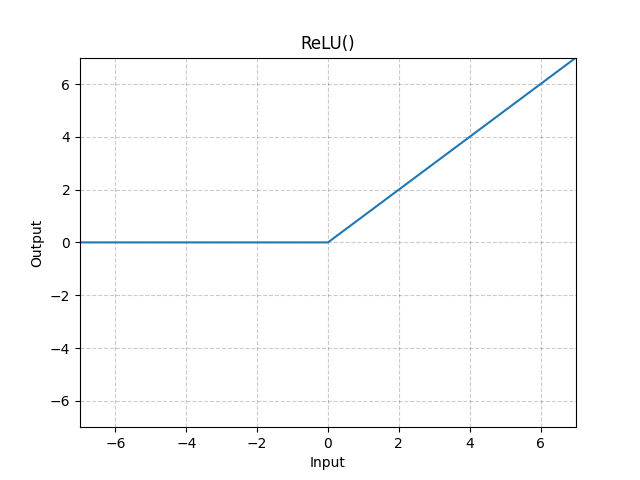
\includegraphics[width=0.75\linewidth]{figures/equations/ReLU.png}
        \caption{Función de activación ReLU.\newline{}Fuente: \href{https://pytorch.org/docs/stable/generated/torch.nn.ReLU.html}{Pytorch torch.nn.ReLU}}
        \label{subfig:torch.nn.ReLU}
    \end{subfigure}
    \hspace{0.02\textwidth} % Espacio horizontal
    \begin{subfigure}{.475\linewidth}
        \centering
        \begin{equation*}\varphi(x) = \operatorname*{max}(0,x)\end{equation*}
        \caption{Función de activación ReLU.\newline{}Fuente: \href{https://pytorch.org/docs/stable/generated/torch.nn.ReLU.html}{Pytorch torch.nn.ReLU}}
        \label{subfig:eq-torch.nn.ReLU}
    \end{subfigure}

    % LeakyReLU
    \medskip % create some *vertical* separation between the graphs
    \begin{subfigure}{.475\linewidth}
        \centering
        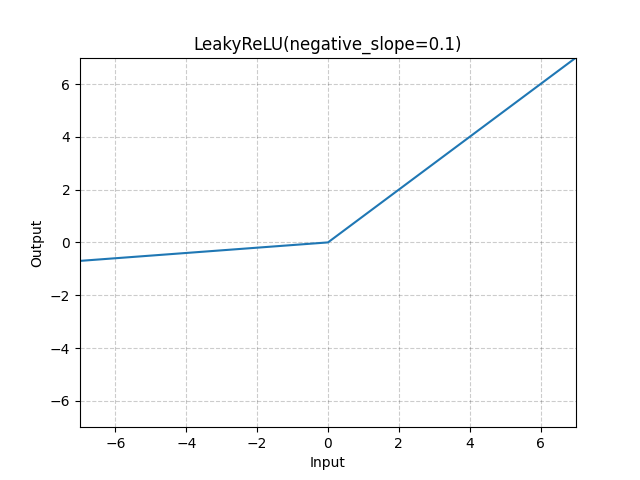
\includegraphics[width=0.75\linewidth]{figures/equations/LeakyReLU.png}
        \caption{Función de activación LeakyReLU.\newline{}Fuente: \href{https://pytorch.org/docs/stable/generated/torch.nn.LeakyReLU.html}{Pytorch torch.nn.LeakyReLU}}
        \label{subfig:torch.nn.LeakyReLU}
    \end{subfigure}
    \hspace{0.02\textwidth} % Espacio horizontal
    \begin{subfigure}{.475\linewidth}
        \centering
        \begin{small}
            \begin{equation*}
                \varphi(x) = \operatorname*{max}\left(0,x\right) + \operatorname*{negative\_slope} * \operatorname*{min}\left(0,x\right)
            \end{equation*}
        \end{small}
        \caption{Función de activación LeakyReLU.\newline{}Fuente: \href{https://pytorch.org/docs/stable/generated/torch.nn.LeakyReLU.html}{Pytorch torch.nn.LeakyReLU}}
        \label{subfig:eq-torch.nn.LeakyReLU}
    \end{subfigure}

    \medskip
    \begin{subfigure}{.475\linewidth}
        \centering
        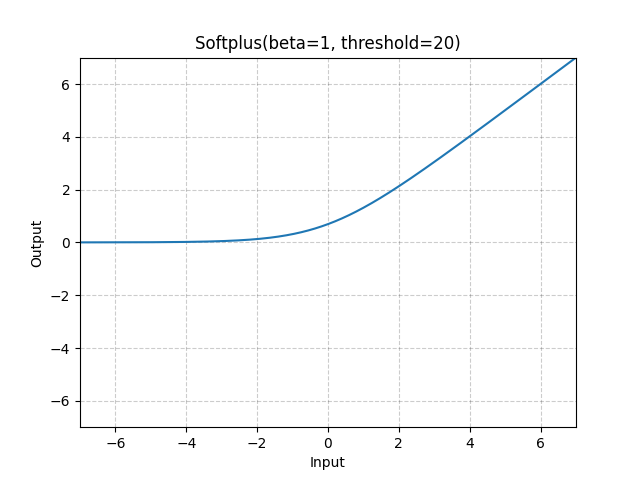
\includegraphics[width=0.75\linewidth]{figures/equations/Softplus.png}
        \caption{Función de activación Softplus.\newline{}Fuente: \href{https://pytorch.org/docs/stable/generated/torch.nn.Softplus.html}{Pytorch torch.nn.Softplus}}
        \label{subfig:torch.nn.Softplus}
    \end{subfigure}
    \hspace{0.02\textwidth} % Espacio horizontal
    \begin{subfigure}{.475\linewidth}
        \centering
        \begin{equation*} \varphi(x) = \frac{1}{\beta} \operatorname*{log}\left(1+e^{\beta x}\right) \end{equation*}
        \caption{Función de activación Softplus.\newline{}Fuente: \href{https://pytorch.org/docs/stable/generated/torch.nn.Softplus.html}{Pytorch torch.nn.Softplus}}
        \label{subfig:eq-torch.nn.Softplus}
    \end{subfigure}

    \caption{Funciones de activación no lineales}
    \label{fig:p1--equations--Non-linear-Activations}
\end{figure}

\begin{figure}[H]
    \centering
    \captionsetup{justification=centering}

    \begin{subfigure}{.475\linewidth}
        \centering
        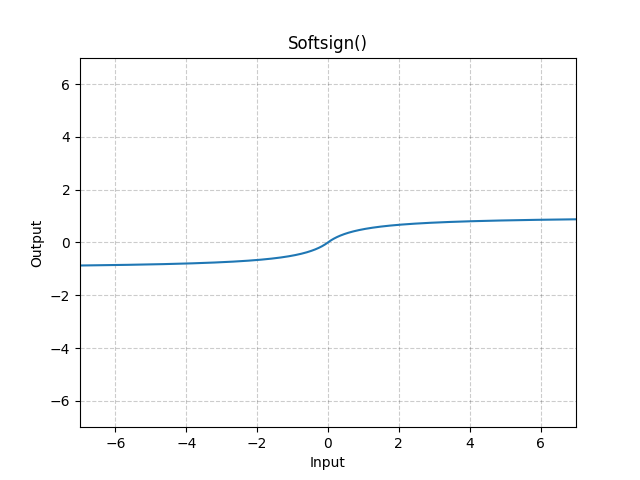
\includegraphics[width=0.75\linewidth]{figures/equations/Softsign.png}
        \caption{Función de activación Softsign.\newline{}Fuente: \href{https://pytorch.org/docs/stable/generated/torch.nn.Softsign.html}{Pytorch torch.nn.Softsign}}
        \label{subfig:torch.nn.Softsign}
    \end{subfigure}
    \hspace{0.02\textwidth} % Espacio horizontal
    \begin{subfigure}{.475\linewidth}
        \centering
        \begin{equation*} \varphi(x) = \frac{x}{1+\lvert x \rvert} \end{equation*}
        \caption{Función de activación Softsign.\newline{}Fuente: \href{https://pytorch.org/docs/stable/generated/torch.nn.Softsign.html}{Pytorch torch.nn.Softsign}}
        \label{subfig:eq-torch.nn.Softsign}
    \end{subfigure}

    % \medskip
    \begin{subfigure}{.475\linewidth}
        \centering
        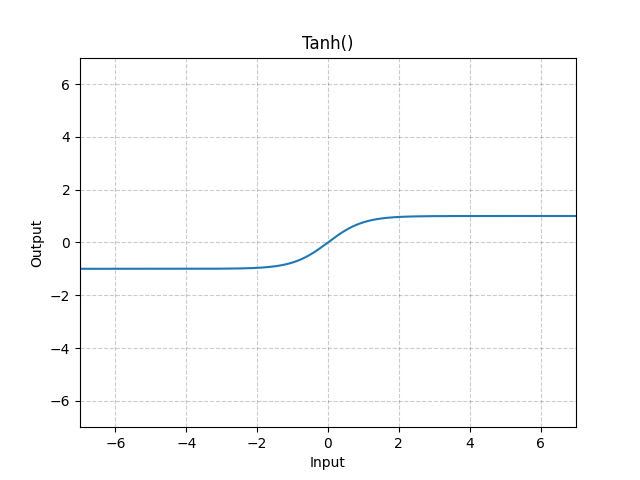
\includegraphics[width=0.75\linewidth]{figures/equations/Tanh.png}
        \caption{Función de activación Tanh.\newline{}Fuente: \href{https://pytorch.org/docs/stable/generated/torch.nn.Tanh.html}{Pytorch torch.nn.Tanh}}
        \label{subfig:torch.nn.Tanh}
    \end{subfigure}
    \hspace{0.02\textwidth} % Espacio horizontal
    \begin{subfigure}{.475\linewidth}
        \centering
        \begin{equation*} \varphi(x) = \frac{e^{x}-e^{-x}}{e^{x}+e^{-x}} \end{equation*}
        \caption{Función de activación Tanh.\newline{}Fuente: \href{https://pytorch.org/docs/stable/generated/torch.nn.Tanh.html}{Pytorch torch.nn.Tanh}}
        \label{subfig:eq-torch.nn.Tanh}
    \end{subfigure}

    % \medskip
    \begin{subfigure}{.475\linewidth}
        \centering
        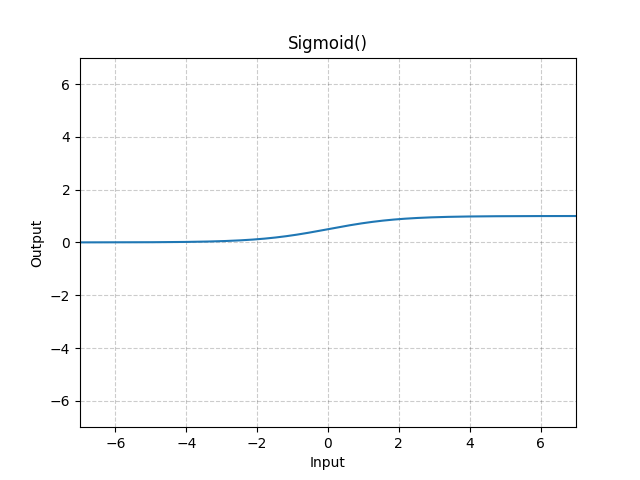
\includegraphics[width=0.75\linewidth]{figures/equations/Sigmoid.png}
        \caption{Función de activación Sigmoid.\newline{}Fuente: \href{https://pytorch.org/docs/stable/generated/torch.nn.Sigmoid.html}{Pytorch torch.nn.Sigmoid}}
        \label{subfig:torch.nn.Sigmoid}
    \end{subfigure}
    \hspace{0.02\textwidth} % Espacio horizontal
    \begin{subfigure}{.475\linewidth}
        \centering
        \begin{equation*} \varphi(x) = \frac{1}{1+e^{-x}} \end{equation*}
        % \label{eq:sigmoid} 
        \caption{Función de activación Sigmoid.\newline{}Fuente: \href{https://pytorch.org/docs/stable/generated/torch.nn.Sigmoid.html}{Pytorch torch.nn.Sigmoid}}
        \label{subfig:eq-torch.nn.Sigmoid}
    \end{subfigure}

    \caption{Funciones de activación no lineales}
    \label{fig:p2--equations--Non-linear-Activations}
\end{figure}


\paragraph*{F. Activaciones no lineales - \textit{Non-linear Activations (other)}}
% TODO: explicar las funciones de activación no lineales más importantes

\begin{enumerate}
    \item \textbf{Softmax}: Aplica la función Softmax a un Tensor de entrada ${n}$-dimensional re-escalándolos para que los elementos del Tensor de salida ${n}$-dimensional se encuentren en el rango [0,1]. \cite{pytorch2024github}
    \item[] \begin{equation} \varphi(x_{i}) = \frac{e^{x_{i}}}{\sum_{j}{e^{x}_{j}}} \end{equation}
    
    % TODO, añadir más si se requiere

% nn.Softmin Applies the Softmin function to an n-dimensional input Tensor. 
% nn.Softmax Applies the Softmax function to an n-dimensional input Tensor. 
% nn.Softmax2d Applies SoftMax over features to each spatial location. 
% nn.LogSoftmax Applies the log ⁡ ( Softmax ( x ) ) log(Softmax(x)) function to an n-dimensional input Tensor. 
% nn.AdaptiveLogSoftmaxWithLoss Efficient softmax approximation.

    
\end{enumerate}


% endregion Funciones de activación

\subsubsection{Tipos de capas}
% region Tipos de capas
% TODO: Capas de entrada, ocultas y de salida.
% TODO: Capas densas, no lineales, con y sin pesos
% TODO: Usos, ventajas y desventajas, paralelización

% Non-linear Activations (weighted sum, nonlinearity)
% Non-linear Activations (other)
% - Convolution Layers
% - Pooling layers
% - Padding Layers
% - Normalization Layers
% - Recurrent Layers
% - Linear Layers
% - Dropout Layers
% - Sparse Layers
% * Distance Functions
% * Loss Functions
% Transformer Layers
% Vision Layers
% Shuffle Layers


Existen una gran variedad de capas con distintos propósitos, permiten organizar y estructurar el funcionamiento de la red durante el proceso de aprendizaje. Cada capa influye con un propósito específico, contribuyendo de manera única al funcionamiento global de la red.

Algunas de las características de los tipos de capas más famosas son las siguientes.

\begin{itemize}
    \item \textbf{Capas densas y dispersas (Denses and Sparses Layers)}:
    \item[]
        \begin{itemize}
            \item \textbf{Capas densas}: Capas que conectan todas las neuronas de una capa con todas las de la capa siguiente.
            \item[] Utilizadas en \acrshort{ANN} tradicionales para tareas de clasificación y regresión.
            \item \textbf{Capas dispersas}: Capas que contienen conexiones dispersas entre neuronas, lo que implica que no todas las neuronas están conectadas entre sí.
            \item[] Se utilizan para reducir la complejidad computacional y el consumo de memoria en grandes modelos.
        \end{itemize}
    \item \textbf{Capas lineales (Linear Layers)}:
    \item[]
        \begin{itemize}
            \item Estas capas generalmente se combinan con funciones de activación no lineales para introducir no linealidad en la red neuronal.
            \item Tanto \texttt{nn.Linear} como \texttt{nn.Bilinear} realizan transformaciones lineales de las entradas ponderando los pesos. \texttt{nn.Identity} no realiza ninguna transformación, y \texttt{nn.LazyLinear} puede realizar transformaciones lineales perezosas.
            \item Proporcionan flexibilidad al permitir ajustar sus parámetros según las necesidades del modelo o la tarea.
        \end{itemize}
    \item \textbf{Capas Convolucionales (Convolutional Layers)}:
          % se especializan en detectar la presencia de características proporcionadas por la entrada del modelo.
    \item[]
        \begin{itemize}
            \item Aplican filtros o convoluciones a la entrada para detectar patrones como bordes, texturas y formas.
            \item Se utilizan principalmente para procesar datos de imágenes y extraer características relevantes.
            \item Son la base del funcionamiento en tareas de clasificación de imágenes o de segmentación de imágenes.
        \end{itemize}
    \item \textbf{Capas de Pooling (Pooling Layers)}:
          % se especializan en comprimir la información de las imágenes preservando la abstracción de las características más importantes, ayudan a reducir el {overfitting}, existen múltiples variantes cómo \texttt{nn.MaxPool1d} o \texttt{nn.AvgPool1d}.
    \item[]
        \begin{itemize}
            \item Comprimen la dimensionalidad de las características extraídas de las capas convolucionales. Se usan entre capas convolucionales.
            \item Existen múltiples variantes cómo \texttt{nn.MaxPool1d} o \texttt{nn.AvgPool1d} que seleccionan los valores más significativos de una región dada.
            \item Ayudan a reducir el {overfitting}, simplificar la representación de características, reducir el coste computacional, etc.
        \end{itemize}
    \item \textbf{Capas de Padding (Paddings Layers)}:
          % se usan para ajustar las dimensiones de los datos de entrada para que sean compatibles con ciertas operaciones, mejoran el rendimiento.
    \item[]
        \begin{itemize}
            \item Se usan para ajustar las dimensiones de los datos de entrada, permiten después aplicar operaciones.
            \item Añade ceros o constantes alrededor de los bordes de regiones para ajustar el tamaño a posteriores operaciones.
            \item Previenen la pérdida de información en los bordes.
        \end{itemize}
    \item \textbf{Capas de Normalización (Normalization Layers)}:
          % se usan para mejorar el rendimiento y la estabilidad del entrenamiento, realizan operaciones sobre los mapas de activación, existen variantes, las más usadas son \texttt{nn.BatchNorm1d} y \texttt{nn.LayerNorm} que permiten aplicar una normalización por lotes o por capas respectivamente.
    \item[]
        \begin{itemize}
            \item Realizan operaciones sobre los mapas de activación, se utilizan para estabilizar y acelerar el entrenamiento de la red.
            \item Algunas de las capas relevantes son \texttt{nn.BatchNorm1d} y \texttt{nn.LayerNorm}, estás permiten aplicar una normalización por lotes o por capas respectivamente.
            \item Ayudan a mantener la distribución de activaciones más consistentes durante el entrenamiento.
        \end{itemize}
    \item \textbf{Capas de Dropout (Dropout Layers)}:
          % se usan para entrenamientos más estables eliminando dependencias, evitan el sobreajuste {overfitting}, esto lo hacen desactivando de forma estocástica ciertas neuronas en las distintas iteraciones.
    \item[]
        \begin{itemize}
            \item Se desactivan aleatoriamente un porcentaje de neuronas en la capa, esto evita dependencias en el entrenamiento, además de generalizar mejor.
            \item Es una técnica de regularización que reduce el sobreajuste, se usan para entrenamientos más estables eliminando dependencias.
        \end{itemize}
    \item \textbf{Capas Recurrentes (Recurrent Layers)}:
          % se usan para procesar datos secuenciales o de series temporales, su característica principal son que tienen memoria, existen distintas variantes en función de cuando tome el contexto, unidireccionales si solo cuenta el contexto previo o bidireccionales si consideran el previo y posterior. Las más usadas son \texttt{nn.RNN}, \texttt{nn.LSTM} y \texttt{nn.GRU}
    \item[]
        \begin{itemize}
            \item Diseñadas para manejar datos secuenciales o de series temporales.
            \item Incorporan conexiones cíclicas que les permiten propagar información de un paso de tiempo a otro, las más usadas son \texttt{nn.RNN}, \texttt{nn.LSTM} y \texttt{nn.GRU}.
            \item Las capas recurrentes tienen memoria y contexto considerando los estados previos, son útiles para traducción de idiomas, procesamiento del lenguaje natural y reconocimiento de voz.
        \end{itemize}
\end{itemize}

% endregion Tipos de capas 

\subsubsection{Topologías de redes neuronales}
% region topologías
% TODO: explicar la existencia de distintas formas de aplicar las capas de neuronas artificiales y sus resultados
La topología o arquitectura de una red neuronal nos referimos a la organización y disposición de las neuronas en la red, formando capas. Estos parámetros fundamentales determinan cómo se estructura la red.
Se suele considerar el número de capas, número de neuronas por capa, tipo de conexiones (unidireccionales o recurrentes).


\begin{figure}[H]
    \centering
    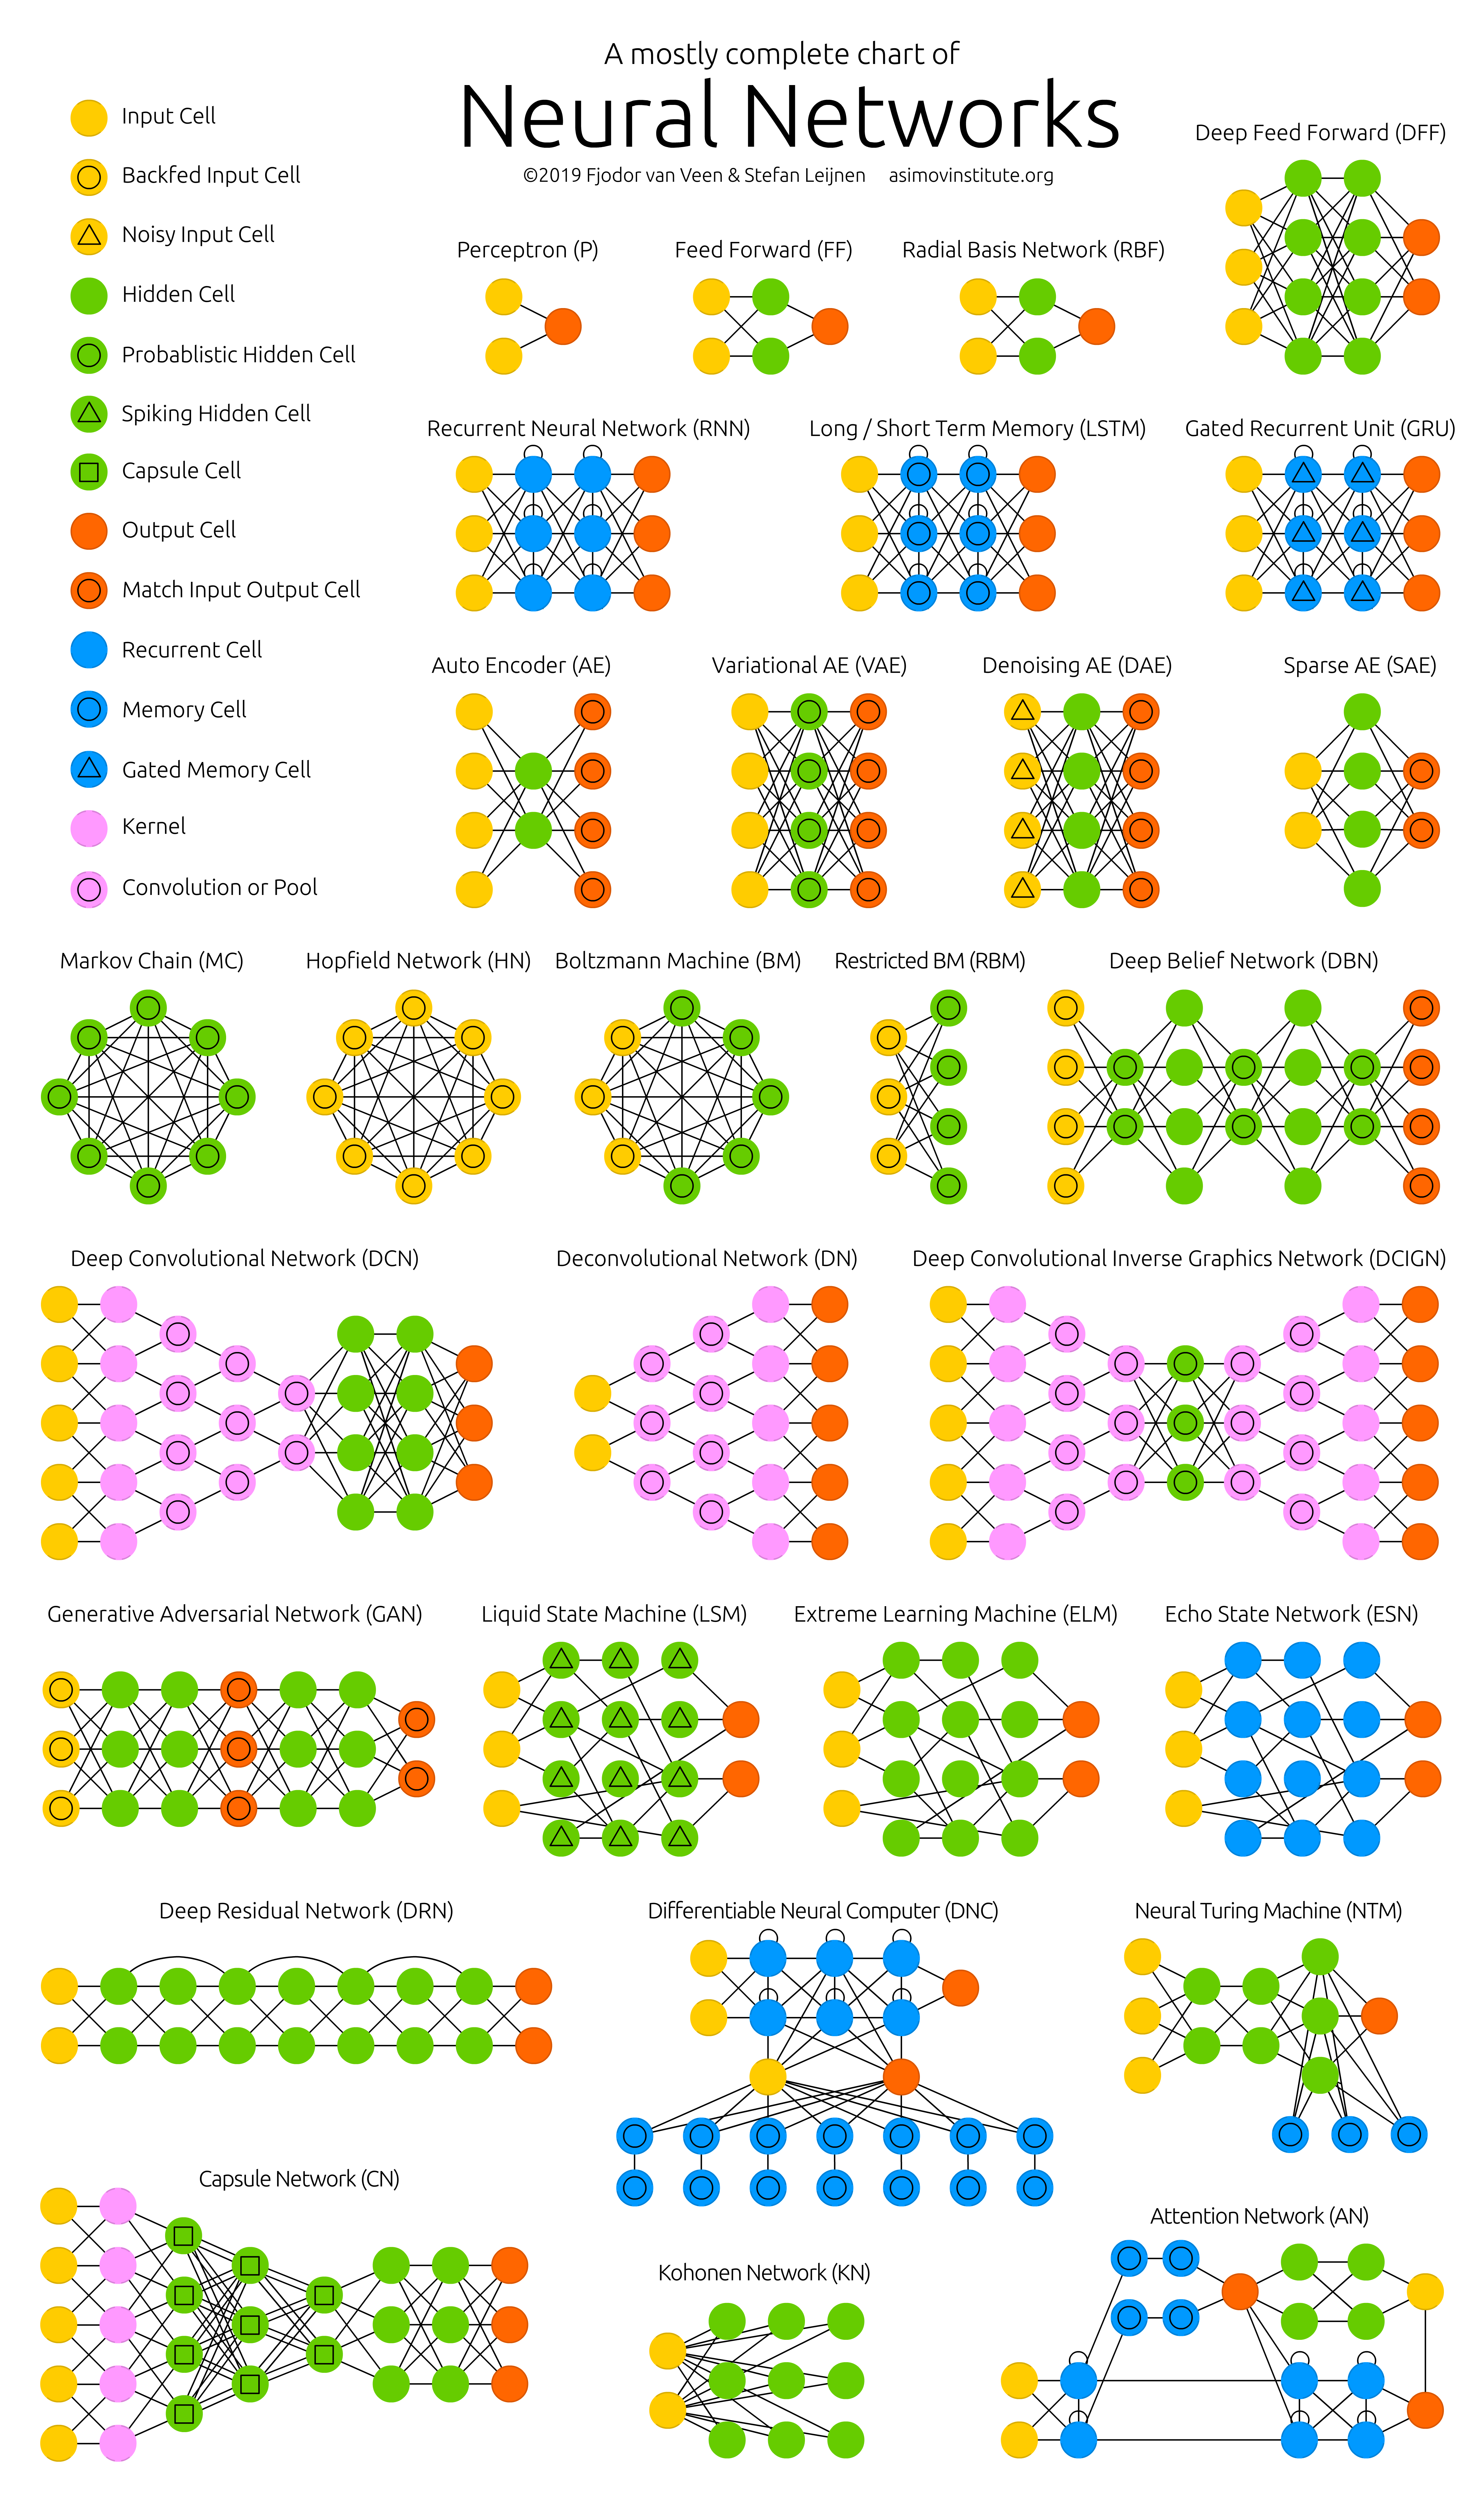
\includegraphics[height=0.95\textheight]{figures/NeuralNetworkZo19High.png}
    \caption{Topologías de redes neuronales.\newline{}Fuente: \href{https://www.asimovinstitute.org/neural-network-zoo/}{The neural network zoo}}
    \label{fig:NeuralNetworkZo19High}
\end{figure}
% endregion topologías


% endregion subsection Redes neuronales artificiales
